\documentclass[12pt]{article}

\author{Groep 6:\\
		Niels Desair\\
		Bram Kelchtermans\\
		Dylan Toirkens}
		
\title{\textbf{Studie van meetbare objectieven en ontwerpprincipes van Shneiderman}}

\date{12/10/2016}

\usepackage{graphicx}
\usepackage{parskip}
\usepackage{float}

\setcounter{tocdepth}{3}
\setcounter{secnumdepth}{3}

\begin{document}
	\begin{titlepage}
		
		\newcommand{\HRule}{\rule{\linewidth}{0.5mm}} % Defines a new command for the horizontal lines, change thickness here
		
		\begin{center} % Center everything on the page
			
			\textsc{\LARGE Universiteit Hasselt}\\[1.5cm] % Nme of your university/college
			\textsc{\Large Humane en sociale aspecten van de informatica}\\[0.5cm] % Major heading such as course name
			
			\HRule \\[0.4cm]
			{ \huge \bfseries Studie van meetbare objectieven en ontwerpprincipes van Shneiderman}\\[0.4cm]
			\HRule \\[1.5cm]
			
			\begin{minipage}{0.4\textwidth}
				\begin{flushleft} \large
					\emph{Groep 6:}\\
					Niels \textsc{Desair} \newline
					Bram \textsc{Kelchtermans} \newline
					Dylan \textsc{Toirkens}
				\end{flushleft}
			\end{minipage}
			~
			\begin{minipage}{0.4\textwidth}
				\begin{flushright} \large
					\emph{Datum:}\\
					12 Oktober 2016
					\emph{Academiejaar: } \\
					2016-2017
				\end{flushright}
			\end{minipage}\\[3cm]
			\vspace{25 mm}
			
\includegraphics[width=3.0cm]{UHasselt-logo.jpg}\\[2.0cm]  
		\end{center}
	\end{titlepage}

\newpage
\tableofcontents
\section{Inleiding}
In deze studie willen wij kijken of een computerprogramma dat dagelijks door duizenden mensen gebruikt wordt goed scoort bij de meetbare objectieven en de principes van Shneiderman. Het programma dat we hiervoor gekozen hebben, is Google Chrome. Deze browser is al enkele jaren de populairste en geniet van een zeer groot aantal gebruikers en wij denken dat de User Interface daar wel iets mee te maken zou kunnen hebben.
\newpage

\section{Bespreking Niels}
\subsection{Meetbare objectieven}
Allereerst begin ik met het bespreken van de 3 meetbare objectieven die ik het belangrijkst vind in een internet browser. Allereerst is dat de subjectieve satisfaction voor mij, gevolgd door de speed of performance en dan de rate of errors by users.
\subsubsection{Subjective satisfaction}
Door de hoeveelheid aan alternatieven voor Google Chrome, die eveneens gratis zijn (denk aan software als Firefox, Opera en Safari) heeft de gebruiker zeer veel keuze. Hierdoor is het belangrijk dat Chrome goed scoort in de subjective satisfaction; als Chrome dit niet doet zal de gebruiker namelijk overstappen naar een concurrent! Het is een feit dat Chrome hier een zeer goede zaak doet, te zien door het feit dat in augusts 2016 meer dan 50\% van alle desktops kozen voor Google Chrome.\cite{NetShare}
\subsubsection{Rate of errors by users}
Een internetbrowser wordt gebruikt om websites te bezoeken, niet om bij iedere stap foutmelding na foutmelding te krijgen en deze telkens op te moeten lossen. In een ideale wereld zou er dus geen errors zijn tenzij de gebruiker echt iets fout doet. Chrome speelt hier op in: zo zal er een poging gedaan worden om fouten van gebruikers automatisch te corrigeren. Typt een gebruiker een fout in de site in de adresbalk, zal Google zelf een zoekopdracht uitvoeren om zo hopelijk toch de gebruiker de juiste weg op te helpen. Dit valt te zien in figuur \ref{fig:search}.
\begin{figure}
	\centering
	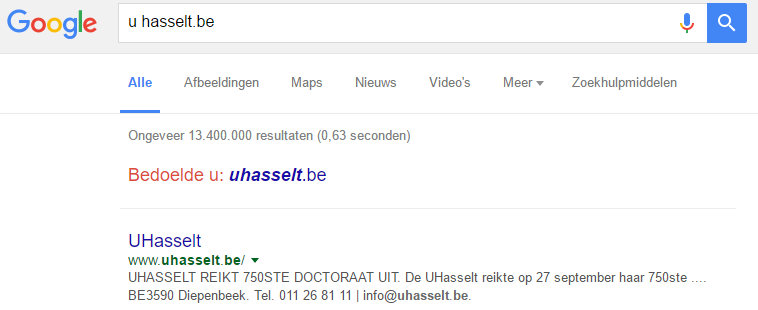
\includegraphics[width=1\textwidth]{search.png}
	\caption{Spatie in URL, Google zoekt de juiste site}
	\label{fig:search}
\end{figure}
\newpage
\subsubsection{Speed of Performance}
Voor mij is het belangrijk dat ik tijdens het browsen van het internet zo weinig mogelijk tijd spendeer aan de browser, en zo veel mogelijk aan de websites die ik wil bekijken. Chrome vergemakkelijkt dit door een enorme hoeveelheid shortcuts (Een 50 tal shortcuts die standaard zijn inbegrepen\cite{shortcuts}) alsook auto-complete bij vaak bezochte websites (figuur \ref{fig:autocomplete}). Dit zorgt ervoor dat men minder tijd moet spenderen aan Chrome, en meer tijd heeft voor de websites die bezocht worden.
\begin{figure}
	\centering
	
\includegraphics[width=0.7\textwidth]{autocomplete.png}
	\caption{Bij het intikken van de 9 vult Chrome de rest aan}
	\label{fig:autocomplete}
\end{figure}

\subsection{Ontwerpprincipes van Shneiderman}
Nu ik mijn mening heb gegeven over de belangrijkste meetbare objectieven, ga ik specifiek kijken naar de User Interface (UI) van Chrome. Deze ga ik bespreken volgens de ontwerpprincipes van Shneiderman en zal ik proberen zowel de dingen die Chrome goed doet en minder goed doet te belichten.
\subsubsection{Herken de diversiteit}
Zoals eerder vermeld heeft Google Chrome een marktaandeel van meer dan 50\% bij desktops. Het is dan aanneembaar dat er grote verschillen tussen deze gebruikers zit en dat er dus zowel beginners, gevorderden en expert gebruikers van Chrome te vinden zijn. Beginners kunnen direct aan de slag met Chrome dankzij de gelijkaardigheid met alle andere webbrowsers: wie ooit al een browser gebruikt heeft, zal snel doorhebben wat nodig is. De UI van Chrome is eenvoudig (figuur \ref{fig:smallUI}), er zijn weinig buttons, waardoor de beginnend gebruiker niet in de verwarring komt. Ook voor de intermediate users is Chrome een zeer goede browser, de UI is nog altijd compact, maar de gebruiker kan Chrome aanpassen naar wens door bijvoorbeeld het gebruik van extensies (figuur \ref{fig:extensions}). Wanneer deze gebruikers toch in de war zijn en nog extra referenties nodig hebben kunnen ze terecht bij het uitgebreide helpcentrum van Chrome (figuur \ref{fig:helpcentrum}). Ook expertgebruikers kunnen snel met Chrome werken: zoals eerder vermeld stelt Chrome een 50tal shortcuts tot de beschikking van zijn gebruikers en het bestaan van extensies kan nog meer shortcuts beschikbaar stellen, zo is er bijvoorbeeld een extensie om custom hotkeys te maken (figuur \ref{fig:shortkeys}).
\begin{figure}
	\centering
	
\includegraphics[width=0.8\textwidth]{smallUI.png}
	\caption{Zeer weinig knoppen, overzicht blijft bewaard}
	\label{fig:smallUI}
\end{figure}
\begin{figure}
	\centering
	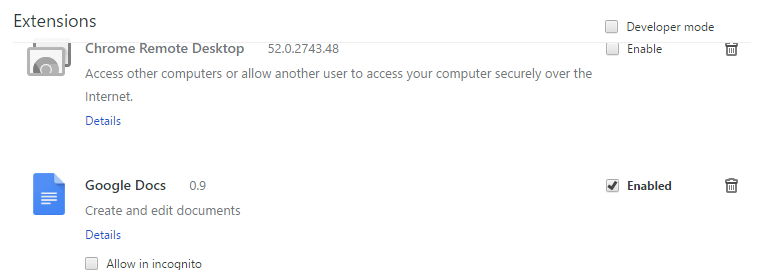
\includegraphics[width=0.9\textwidth]{extensions.png}
	\caption{Chrome naar eigen voorkeur aanpassen met extensions}
	\label{fig:extensions}
\end{figure}
\begin{figure}
	\centering
	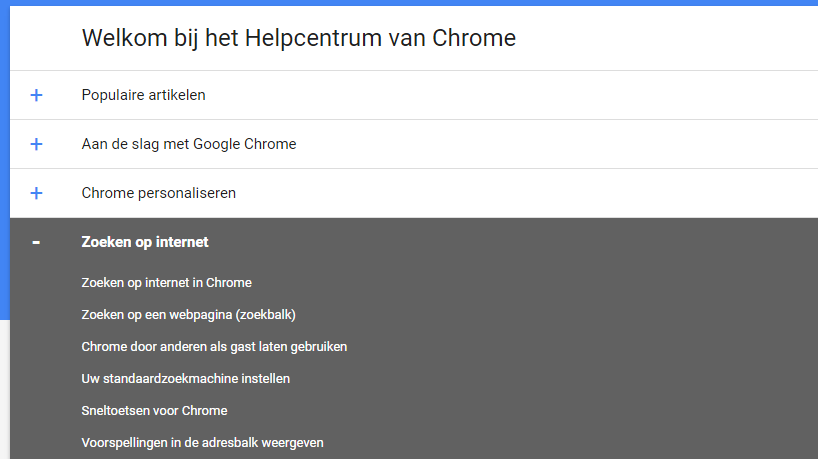
\includegraphics[width=0.8\textwidth]{helpcentrum.png}
	\caption{Uitgebreid helpcentrum met tal van artikels}
	\label{fig:helpcentrum}
\end{figure}
\begin{figure}
	\centering
	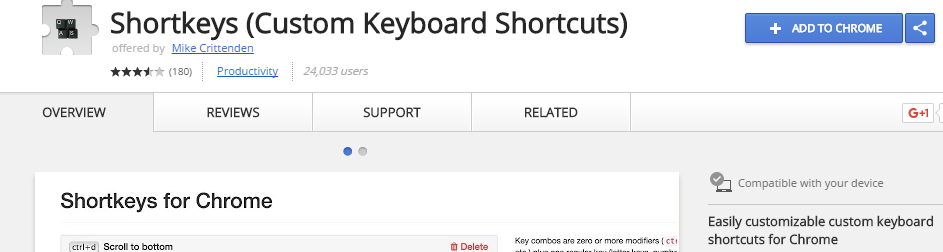
\includegraphics[width=0.8\textwidth]{shortkeys.png}
	\caption{Extensie waarmee de gebruiker zelf keyboard shortcuts kan maken}
	\label{fig:shortkeys}
\end{figure}
\subsubsection{De acht gouden regels voor interface design}
\begin{itemize}
	\item Streven naar consistentie
	\newline
	Chrome is zeer consistent met andere browsers, dit door het gebruik maken van icoontjes op knoppen die overeen komen met dezelfde knoppen in andere browsers. Denk aan de ster van bladwijzers/favorieten, de pijltjes voor vorige (figuur \ref{fig:back}) of volgende pagina enzovoorts. Binnen Chrome zelf is het moeilijker om consistentie te garanderen: de websites nemen namelijk zelf een groot deel van de schermruimte in beslag. Wat Chrome wel doet is telkens dezelfde grijstinten gebruiken binnen de UI, waardoor het een samenhangend geheel blijft.
	\begin{figure}
		\centering
		
\includegraphics[width=0.1\textwidth]{back.png}
		\caption{Terugkeerpijltjes in Chrome (links) en Firefox (rechts)}
		\label{fig:back}
	\end{figure}
	\item Frequente gebruikers toelaten schortcuts te gebruiken
	\newline
	Er zijn tal van shortcuts aanwezig vanaf de installatie, een 50 tal toetsencombinaties\cite{shortcuts} en de optie om er nog extra te maken. Een minpuntje hierbij is wel dat er extensies moeten ge\"installeerd worden om deze extra shortcuts te gebruiken, aangezien deze niet standaard in Chrome zitten.
	\item Informatieve feedback aanbieden
	\newline
	Chrome slaagt er in om zeer duidelijk feedback te bieden. Zo is er nooit twijfel wanneer er iets fout loopt en kan de gebruiker altijd zijn progressie zien. Enkele voorbeelden hiervan is de duidelijke progresbalk bij het downloaden, het draaiende cirkeltje bij het laden van een pagina en de totale verandering van thema en een duidelijke melding wanneer men incognitomode gebruikt (figuur \ref{fig:incognito}).
	\newpage
	\begin{figure}
		\centering
		
\includegraphics[width=0.8\textwidth]{incognito.png}
		\caption{Verandering van thema en melding bij incognitomode}
		\label{fig:incognito}
	\end{figure}
	\item Dialogen ontwerpen zodat onverwachte resultaten uitgesloten worden en de voortgang duidelijk is
	\newline
	Het kan al eens gebeuren dat men verkeerd klikt en per ongeluk een tabblad sluit in plaats van eentje te openen, in dit geval zal Chrome geen dialoog gebruiken om dit te voorkomen. Zelfs bij het sluiten van de browser met meerdere tabbladen open zal er geen bevestiging gevraagd worden door Chrome, wat concurrent Firefox wel doet. Dit is een element waar Chrome nog op kan verbeteren. In sommige andere gevallen, zoals bevestiging vragen bij het sluiten van Chrome tijdens een download, is er wel een dialoog bij Chrome (figuur \ref{fig:dl}). 	
	\begin{figure}
		\centering
		
\includegraphics[width=0.7\textwidth]{imgDownload.png}
		\caption{Bevestiging vragen bij het sluiten van Chrome tijdens een download}
		\label{fig:dl}
	\end{figure}
	\item Foutenpreventie
	\newline
	In plaats van een error te geven, zal Chrome bij het intikken van iets dat geen URL is in de adresbar kiezen om een zoekopdracht naar deze term te doen, om zo gebruikersfouten te vermijden. Verder blijft het zo dat Chrome een webbrowser is, waar zeer weinig fouten in kunnen gebeuren.
	\newpage
	\item Acties omkeerbaar maken
	\newline
	Men kan ten allen tijden terug naar de vorige pagina gaan wanneer men op een verkeerde link klikt. Via het geschiedenis venster kan men zelfs veel verder terug gaan om zo verder terug te gaan (figuur \ref{fig:history}). Ook zijn er shortcuts die acties omkeren: zo zal ctrl+shift+t het laatste gesloten tabblad herstellen. Dit is een klein minpuntje, aangezien het jammer is dat zo'n nuttige functie achter een shortcut zit is het in te denken dat een redelijk deel van gebruikers deze niet kennen en deze functie dus niet kunnen gebruiken.
	\begin{figure}
		\centering
		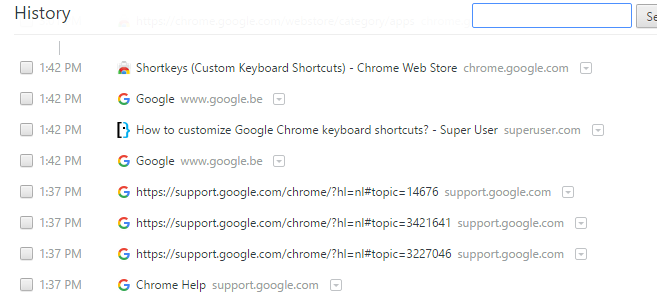
\includegraphics[width=1\textwidth]{history.png}
		\caption{De lijst van bezochte websites, met 1 klik kan een website terug bezocht worden van hier}
		\label{fig:history}
	\end{figure}
	\item Gebruiker meester over het systeem laten zijn
	\newline
	Chrome is zeer aanpasbaar aan de eisen van de gebruiker, vooral door het ondersteunen van extensies. Hiermee kan de gebruiker zijn surfervaring met Chrome aanpassen zoals hij wilt, en dankzij het bestaan van duizenden extensies is de kans groot dat de gebruiker zijn zin zal vinden. \cite{extensions}
	\item Aantal gegevens beperken die de gebruiker moet onthouden
	\newline
	Chrome blijft een simpele UI hebben, waardoor de gegevens die een gebruiker moet onthouden klein zijn. Het enige punt waar er meer moeite nodig is, is bij shortcuts, en aangezien dit iets voor expert users is, is dat verder geen probleem.
	\end{itemize}
\newpage

\section{Bespreking Bram}
In dit deel bespreekt Bram Kelchtermans zijn bevindingen over de gekozen software. Als meetbare human-factor objectieven heeft hij gekozen voor "Subjective satisfaction", "Speed of Performance" en "Error Rate". Verder wordt er ook nog gesproken over de "Ontwerpprincipes van Shneiderman" toegepast op de gekozen software.
\subsection{Meetbare objectieven}
\subsubsection{Subjective Satisfaction}
Voor de meetbare human-factors objectieven heb ik "subjective satisfaction" gekozen als het belangrijkste aspect. Dit omdat er veel concurrentie is op het vlak van webbrowsers, hierbij zijn zo goed als alle webbrowsers gratis. Daardoor is het dus belangrijk dat de gebruikers tevreden zijn over het ontwerp en de werking van Chrome als Google wil dat Chrome consistent gebruikt blijft worden. De gebruiker kan namelijk gemakkelijk en gratis overstappen naar een alternatief zoals bijvoorbeeld Mozilla Firefox. Het lijkt me dus duidelijk dat dit een zeer belangrijk objectief is om na te streven door de ontwerpers. Persoonlijk vind ik dat Google hier zeker op vooruit is gegaan. Dit doordat ze de mogelijkheid geven aan de gebruikers om Chrome aan te passen naar zijn of haar voorkeuren. Denk zo maar aan de ad-block software die er voor zorgt dat alle reclame op sites verdwijnt. Dit is voor vele gebruikers een rede om Chrome te gebruiken. 
\subsubsection{Speed of Performance}
Een ander belangrijk aspect vind ik persoonlijk de "speed of performance". Als we de verschillende gebruikers bekijken bekomen we dat we zowel particulieren als commerci\"ele gebruikers hebben. Het is dus zeer belangrijk voor beide groepen dat het programma dus een snelle verbinding tot het wereldwijde web voorziet. Zoals hierboven al besproken is, kan de gebruiker makkelijk overstappen naar de concurrent als deze sneller is. Op dit vlak is Chrome nog steeds één van de pioniers. Een nadeel is echter dat de eventueel geïnstalleerde plugins en extensions er voor kunnen zorgen dat het surfen minder vlot verloopt. Een goed voorbeeld van dit probleem is de Hangouts extensie. Wanneer deze ge\"installeerd is, werkt Chrome aanzienlijk trager waardoor de gebruiker geneigd zal zijn deze extensie te verwijderen.
\subsubsection{Error Rate}
Tenslotte zou ik het nog willen hebben over de "error rate" van Chrome. Het is belangrijk dat er zo weinig mogelijk fouten optreden bij het gebruik van een webbrowser. Wanneer het programma bijvoorbeeld crasht bij een bepaalde actie zal de gebruiker zich snel genoodzaakt voelen om een alternatief te vinden. Uit persoonlijke ervaring kan ik zeggen dat er meer fouten optreden bij het gebruik van Chrome als vroeger. Persoonlijk denk ik dat dit komt door een te groot aanbod aan extensies en plugins. Dit kan er voor zorgen dat bij het openen van bepaalde sites het programma crasht doordat een plugin niet goed werkt of vast loopt.
\subsection{Ontwerpprincipes van Shneiderman}
\subsubsection{Herken de diversiteit}
Er zijn veel gebruikersgroepen als we het hebben over webbrowsers. Zowel particulieren als bedrijven maken vaak gebruik van webbrowsers. In deze twee groepen kunnen we dan weer onderscheid maken in beginnende gebruikers, gebruikers met gemiddelde kennis en expert gebruikers. 
\linebreak
Beginnende gebruikers zullen eerst moeten leren hoe een webbrowser werkt. Dit heeft echt weinig tot geen gevolgen voor de gebruiksfactor van Chrome. Dit doordat elke webbrowser via hetzelfde principe werkt en dus altijd aangeleerd zal moeten worden. Er wordt dus geen risico gelopen dat beginnende gebruikers zullen overstappen naar de concurrent. Voor beginnende gebruikers voorzien ze wel de nodige feedback, dit speelt zeker in het voordeel van Chrome. Denk maar aan de hulp die Chrome biedt wanneer de gebruiker internetproblemen heeft, zoals te zien is in Figuur \ref{fig:nocon}.
\begin{figure}
  \centering
    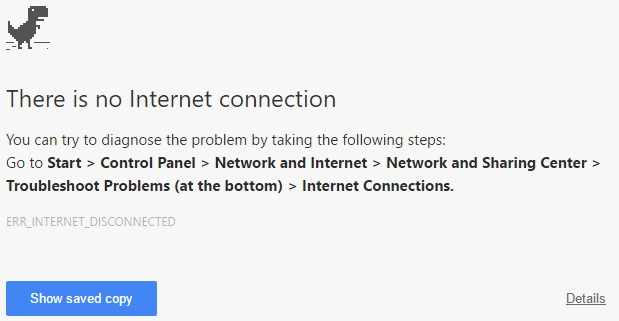
\includegraphics[width=0.7\textwidth]{NoConnection.jpg}
  \caption{Gebruiker heeft geen internetverbinding}
  \label{fig:nocon}
\end{figure}
Deze melding geeft in stappen weer wat de gebruiker moet doen om het probleem op te lossen. Beginnende gebruikers kunnen deze informatie zeker gebruiken en dit speelt dan ook in het voordeel van Chrome.
\newpage
Gebruikers die al wat ervaring hebben met surfen op het web zullen ook sneller de voorkeur geven aan Chrome. Dit doordat Chrome zeer simplistisch is als we over de lay-out spreken. Voor de verdere functionaliteiten moet de gebruiker in de menu's navigeren, ook zijn er speciaal voorziene pagina's (zoals de pagina die te zien is in Figuur \ref{fig:apps}). De gebruiker die meer uit zijn of haar browser wil halen kan op deze pagina terecht om de functionaliteiten uit te bereiden. Zo komen we bij de gebruikers die al veel ervaring hebben met Chrome
\newline
Gebruikers die Chrome al lange tijd gebruiken zullen meer functionaliteiten ter beschikking kunnen krijgen als zij dat willen. Denk zo maar aan Gmail, Google Drive... al deze applicaties zijn geoptimaliseerd voor Chrome. Een ander groot voordeel dat de gebruikers zullen ondervinden is het feit dat Chrome de mogelijkheid biedt om de gegevens te synchroniseren tussen de verschillende apparaten. Denk zo maar aan de surf geschiedenis die ook te vinden zal zijn op de mobiele telefoon van de gebruiker. Dit speelt zeker in het voordeel van Chrome. Gebruikers krijgen ook de mogelijkheid om plugins te installeren om het surfen aangenamer te maken, dit is echter niet essentieel. Beginnende gebruikers kunnen profiteren van de snelheid die Chrome biedt, terwijl Chrome voor expert gebruikers de mogelijkheid biedt om de browser aan te passen aan de verschillende eisen van de gebruikers.
\begin{figure}
  \centering
    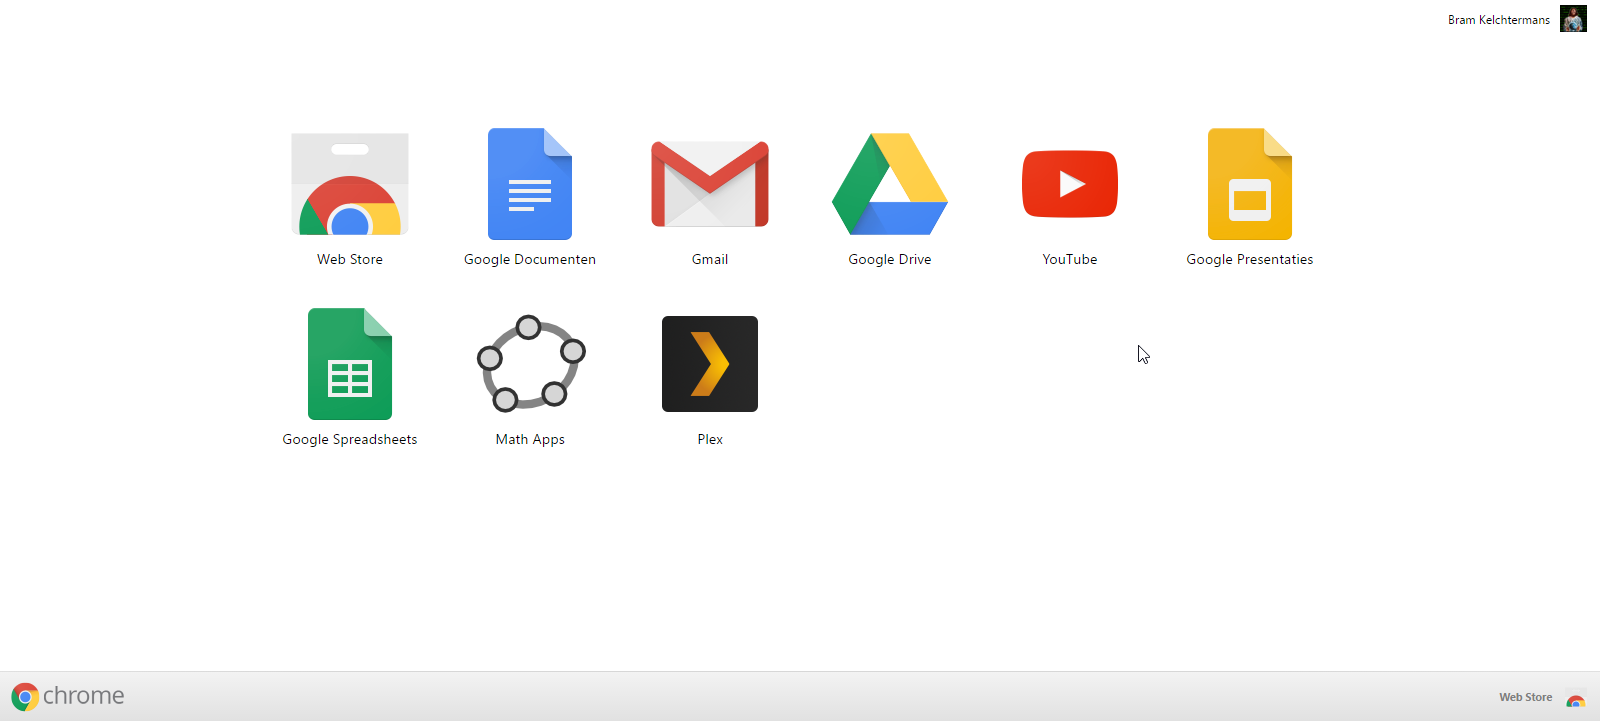
\includegraphics[width=0.9\textwidth]{apps.png}
  \caption{Applicatie pagina van Chrome}
  \label{fig:apps}
\end{figure}
\newpage
\subsubsection{De acht gouden regels voor interface design}
\begin{itemize}
\item Streven naar consistentie
\newline
Bij browsers is het belangrijk dat er consistent gebruik wordt gemaakt van zowel de lay-out als de gebruikte icoontjes. Dit is zeker het geval, zoals te zien is in Figuur \ref{fig:tabsChrome}. Zoals in elke webbrowser wordt er gebruik gemaakt van dezelfde lay-out om verschillende tabbladen aan te geven of de adresbalk te tonen. Dit is belangrijk doordat de gebruiker hierdoor het programma sneller leert te gebruiken.
\begin{figure}
  \centering
    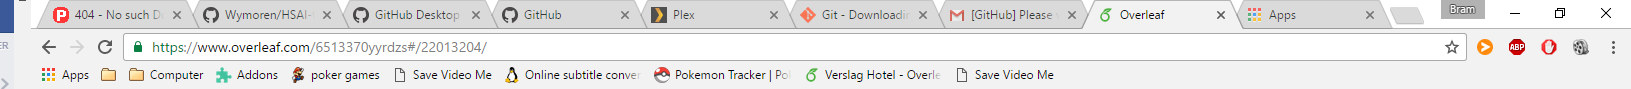
\includegraphics[width=0.9\textwidth]{Tabs_Chrome.png}
  \caption{Het lint van Chrome}
  \label{fig:tabsChrome}
\end{figure}
\item Frequente gebruikers toelaten schortcuts te gebruiken
\newline
De gebruikers kunnen hun favoriete pagina's opslaan als bladwijzers. Deze zijn terug te vinden onder de adresbalk (zie Figuur \ref{fig:tabsChrome}). Dit zorgt er voor dat belangrijke pagina's snel toegankelijk zijn, hierdoor wordt de effici\"entie verhoogd.
\item Informatieve feedback aanbieden
\newline
Een voorbeeld hier van is te zien in afbeelding \ref{fig:nochanges}. De gebruiker probeert hier de pagina te verversen terwijl er een wijziging is aangebracht op de pagina die niet bevestigd is. In dit geval wil de gebruiker een post plaatsen op Facebook maar heeft deze nog niet ingediend. Chrome geeft hier een melding van zodat de gebruiker geen data verliest.
\begin{figure}
  \centering
    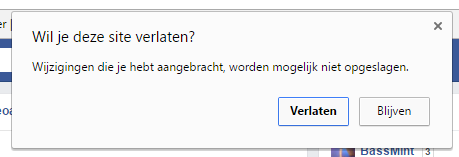
\includegraphics[width=0.9\textwidth]{No_Changes.png}
  \caption{Feedback in Chrome}
  \label{fig:nochanges}
\end{figure}
\newpage
\item Dialogen ontwerpen zodat onverwachte resultaten uitgesloten worden en de voortgang duidelijk is.
\newline
In het vorige puntje wordt er al een dergelijk dialoog besproken.
Een ander voorbeeld van dit puntje is te vinden in Figuur \ref{fig:privatecon}. De gebruiker krijgt hier een melding dat de site niet veilig is voor de privacy van de gebruiker. De gebruiker krijgt echter wel nog de mogelijkheid om verder te surfen naar de gekozen website door op "Advanced" te klikken. Zo weet de gebruiker dat Chrome niet garandeerd dat zijn of haar privacy veilig is.
\newline
\begin{figure}
  \centering
    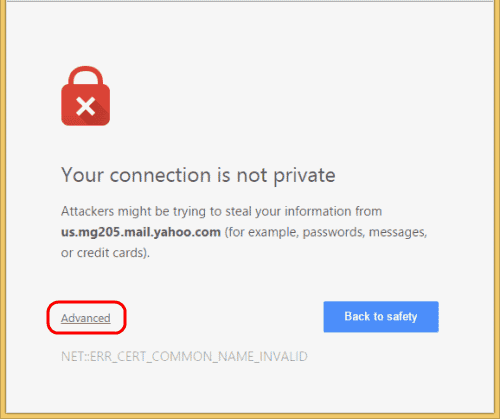
\includegraphics[width=0.9\textwidth]{Chrome-Advanced.png}
  \caption{Onveilige pagina in Chrome}
  \label{fig:privatecon}
\end{figure}
Een ander voorbeeld is te zien in Figuur \ref{fig:loading}, hier kan de gebruiker zien dat de gevraagde pagina geladen wordt. Dit doordat naast de naam van de pagina een laad icoontje te zien is. Hierdoor weet de gebruiker dat hij of zij nog even moet wachten om het gewenste resultaat te bekomen.
\begin{figure}
  \centering
    
\includegraphics[width=0.4\textwidth]{Loading.png}
  \caption{Pagina laden in Chrome}
  \label{fig:loading}
\end{figure}
\item Foutpreventie 
\newline
Een voorbeeldje hier van is niet makkelijk te vinden. Het is logisch dat een webbrowser zo vlot mogelijk moet werken en dus weinig fouten mag genereren. Wat bij Chrome een voordeel is, is de integratie van de zoekmachine in de adresbalk. Dit kan gezien worden als foutpreventie. In een situatie waar de gebruiker een schrijffout maakt in zijn of haar URL wordt dit automatisch gezocht op Google en zo kan er dus een verbetering komen. Zo wordt er vermeden dat een onbestaande pagina geopend wordt.
\item Acties omkeerbaar maken
\newline
Het meest voor de hand liggende voorbeeld is natuurlijk de pijl naar links om naar de vorige pagina te gaan. De gebruiker kan zo terug gaan naar de vorige pagina en dus een actie omkeren.
\item Gebruiker meester over het systeem laten zijn
\newline
Door de integratie van plugins en extensies kan de gebruiker Chrome zodanig aanpassen naar eigen voorkeuren. Dit zorgt er voor dat de gebruiker het gevoel krijgt het hele programma in handen te hebben. Dit is zeker een groot voordeel aan Chrome.
\item Gegevens beperken dat de gebruiker moet onthouden
\newline
Voor het basisgebruik van Chrome zijn er niet veel gegevens die onthouden moeten worden. Wanneer de gebruiker echter verder wilt profiteren van de voordelen van Chrome zijn er hier en daar toch een paar dingen die onthouden moeten worden. Denk zo aan het proces om een extensie toe te voegen aan Chrome.
\end{itemize}
\newpage

\section{Bespreking Dylan}
In dit deel ga ik "Subjective satisfaction", "Speed of Performance" en "Rate of errors by users" bespreken als de meetbare human-factor objectieven. Vervolgens worden de eerste 2 ontwerpprincipes van Shneiderman besproken.
\subsection{Meetbare objectieven}
\subsubsection{Subjective satisfaction}
Naar mijn mening is "subjective satisfaction" het belangrijkste meetbare objectief bij de keuze van een browser. Het is namelijk gemakkelijk om naar een andere browser over te stappen aangezien alle browsers gratis aangeboden worden. Hierdoor moet er voldoende aandacht besteed worden aan het ontwerp en het gebruiksgemak van van een browser. Google Chrome doet het op dit vlak goed. De UI is zeer simpel, bestaande uit enkel een adresbalk, een paar knoppen en eventueel een bladwijzerbalk zoals te zien in Figuur \ref{fig:simpleUI}. Hiermee worden gebruikers niet geconfronteerd met teveel functies, maar via de instellingen kunnen er nog altijd knoppen toegevoegd of weggehaald worden als dit gewenst is.
\begin{figure}
	\centering
	
\includegraphics[width=0.9\textwidth]{imgSimpleUI.png}
	\caption{Chrome heeft slechts een paar knoppen beschikbaar}
	\label{fig:simpleUI}
\end{figure}
\subsubsection{Speed of performance}
Het volgende aspect dat ik ga bespreken is "speed of performance". Voor de meest voorkomen taken zijn er knoppen voorzien, waardoor je deze taken ook in een beperkt aantal stappen snel kan uitvoeren. Een handige kenmerk bij Chrome is dat je je meest bezochte pagina's kan zien en onmiddelijk kan openen wanneer je een nieuw tabblad opent.
\subsubsection{Rate of errors by users}
Als laatste meetbare objectief heb ik "rate of errors by users" gekozen. Een gebruiker zou liefst geen fouten of vergissingen willen maken bij het uitvoeren van een taak. Deze fouten zouden dan zo gemakkelijk mogelijk opgelost moeten worden. Als een gebruiker bijvoorbeeld een tablad perongeluk sluit, zijn er verschillende mogelijkheden om dit op te lossen. Je kan een nieuw tablad openen en de website opnieuw ingeven in de adresbalk of je kan de website zoeken in je geschiedenis. Beide opties zijn omslachtig omdat ze redelijk veel werk vereisen. Er bestaat ook een sneltoets om je laatst gesloten tabblad te openen, maar deze functie is voor de meeste gebruikers onbekend en er wordt hiervoor ook geen knop voorzien. Dit heeft mogelijk te maken met het simpele UI ontwerp dat Chrome nastreeft.
\subsection{Ontwerpprincipes van Shneiderman}
\subsubsection{Herken de diversiteit}
Als we gebruikers indelen in groepen naargelang hun kennis over webbrowsers, dan kunnen we drie groepen vaststellen: nieuwe gebruikers, gebruikers met een algemene kennis en expert gebruikers. Bij nieuwe gebruikers veronderstel ik dat ze weinig kennis hebben van browsers. Vanwege de simpele UI kan een nieuwe gebruiker niet veel fouten maken en wordt ze niet overdonderd met functies. De verschillende knoppen geven een tooltip over hun functie wanneer de cursor er even op stilstaat. Daarnaast wordt er ook duidelijke feedback verwacht. In Figuur \ref{fig:paginaLaden} zien we de 2 manieren waarop Chrome duidelijk maakt dat een pagina aan het laden is. Naast de naam van de pagina verschijnt een icoontje totdat de pagina geladen is, en de knop om een pagina opnieuw te laden verandert in een kruisje.
\begin{figure}
	\centering
	
\includegraphics[width=0.9\textwidth]{imgPaginaLaden.png}
	\caption{Feedback bij het laden van een pagina}
	\label{fig:paginaLaden}
\end{figure}
\linebreak
Gebruikers met al wat kennis over browsers zullen een voorkeur hebben voor browsers die gemakkelijk te gebruiken zijn. Chrome doet dit goed door de meest gebruikte functies samen te voegen in een menu. 
\linebreak
Gebruikers die Chrome regelmatig gebruiken kiezen deze browser omwille van functies die andere browsers niet aanbieden. Zo biedt Chrome bijvoorbeeld de mogelijkheid om in te loggen op je Google-account. Wanneer je dit doet op meerdere apparaten onder hetzelfde account, kunnen je bladwijzers, geschiedenis en andere instellingen op alle andere apparaten gebruikt worden.

\subsubsection{De acht gouden regels voor interface design}
\begin{itemize}
	\item Streven naar consistentie
	\newline
	Bij browsers is het belangrijk om consistent te zijn voor het gebruiksgemak. Chrome doet dit net zoals andere browsers door het gebruik van dezelfde symbolen en lay-out bij het tonen van knoppen en tabbladen. Ook de sneltoetsen komen in grote mate overeen met andere browsers.
	\item Frequente gebruikers toelaten schortcuts te gebruiken
	\newline
	Een aantal functies kunnen i.p.v. met een knop ook met een sneltoets opgeroepen worden. Chrome laat dit bijvoorbeeld weten bij de knoppen in het menu, zoals te zien is in Figuur \ref{fig:shortcuts}. Verder zijn er nog functies die enkel opgeroepen kunnen worden met bepaalde toetsencombinaties, maar de gebruiker zal deze moeten opzoeken om ze te leren kennen.
	\begin{figure}
		\centering
		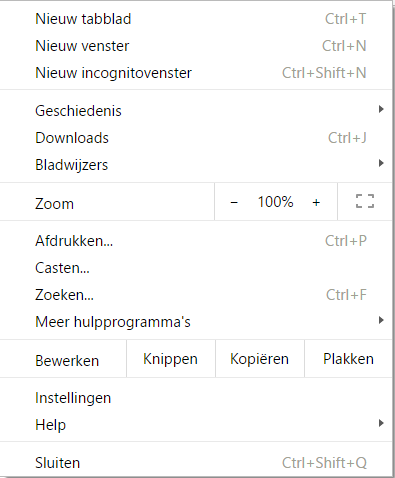
\includegraphics[width=0.4\textwidth]{imgShortcuts.png}
		\caption{Keyboard shortcuts aangeven voor een aantal knoppen in het menu}
		\label{fig:shortcuts}
	\end{figure}
	\item Informatieve feedback aanbieden
	\newline
	Eerder hebben we al aangehaald dat Chrome duidelijk weergeeft wanneer een pagina nog niet geladen is. In Figuur \ref{fig:vertaal} is te zien dat de browser ook een icoon toont wanneer een pagina vertaald kan worden en toont een dialoog wanneer deze vertaald is.
	\begin{figure}
		\centering
		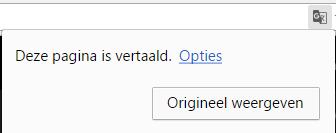
\includegraphics[width=0.4\textwidth]{imgVertaal.png}
		\caption{Webpagina in Chrome vertaald}
		\label{fig:vertaal}
	\end{figure}
	\item Dialogen ontwerpen zodat onverwachte resultaten uitgesloten worden en de voortgang duidelijk is
	\newline
	Wanneer een bestand wordt gedownload, wordt de voortgang onderaan in Chrome getoond. Als de gebruiker Chrome probeert af te sluiten voordat de download afgerond is, wordt de gebruiker hiervan op de hoogte gesteld om dit te bevestigen, zoals te zien is in Figuur \ref{fig:download}.
	\begin{figure}
		\centering
		
\includegraphics[width=0.4\textwidth]{imgDownload.png}
		\caption{Chrome vraagt de gebruiker om bevestiging als de browser afgesloten wordt tijdens het downloaden van een bestand}
		\label{fig:download}
	\end{figure}
	\item Foutenpreventie
	\newline
	Het bovenstaande voorbeeld is ook hier van toepassing. Chrome probeert fouten bij gebruikers te vermijden door ze te melden wanneer een download nog niet is voltooid bij het afsluiten van de browser. Hierdoor is de kans dat een gebruiker dit perongeluk doet kleiner.
	\item Acties omkeerbaar maken
	\newline
	Een voorbeeld hiervan is het ongedaan maken van het verwijderen van een miniatuur bij een nieuw tabblad. Figuur \ref{fig:miniatuur} toont deze optie. Het kan namelijk voorkomen dat een gebruiker een veel gebruikte pagina wilt openen, maar door in de rechterbovenhoek van de miniatuur te klikken, wordt deze uit de lijst verwijderd. Deze vergissing kan ongedaan gemaakt worden in Chrome.
	\begin{figure}
		\centering
		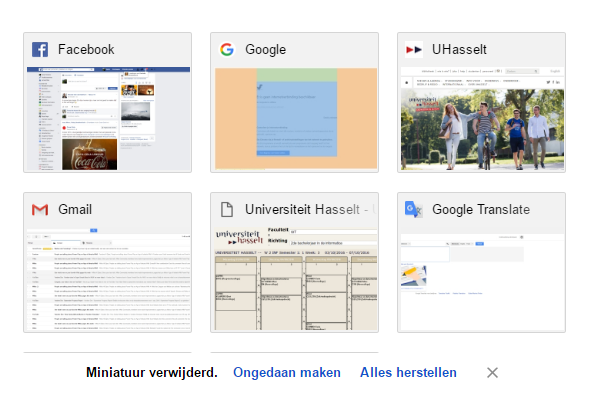
\includegraphics[width=0.9\textwidth]{imgMiniatuur.png}
		\caption{Chrome biedt de mogelijkheid om een verwijderde miniatuur ongedaan te maken}
		\label{fig:miniatuur}
	\end{figure}
	\item Gebruiker meester over het systeem laten zijn
	\newline
	In Figuur \ref{fig:vertaalAltijd} kan je zien dat Chrome de optie biedt om een pagina in een bepaalde taal altijd te vertalen naar een andere taal. 
	\begin{figure}
		\centering
		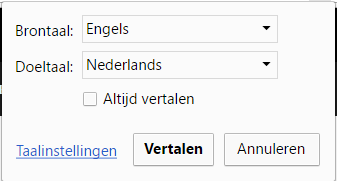
\includegraphics[width=0.4\textwidth]{imgVertaalAltijd.png}
		\caption{Het is mogelijk in Chrome om pagina's in een bepaalde taal altijd te vertalen}
		\label{fig:vertaalAltijd}
	\end{figure}
	\item Gegevens beperken dat de gebruiker moet onthouden
	\newline
	Vanwege de simpele lay-out in Chrome zijn er maar weinig gegevens die een gebruiker hierover moet onthouden. Een gebruiker zou zich ook na lange tijd kunnen herinneren wat en waar de meeste functies te vinden zijn.
\end{itemize}
\newpage


\section{Conclusie}
Nu we alle 3 onze eigen interpretatie en mening gegeven hebben, is het tijd om gezamelijk tot een conclusie te komen. Dit was echter makkelijker dan gedacht, aangezien we op zo goed als ieder punt dezelfde mening hebben. Zo vullen we elkaar aan en was de discussie aangenaam en constructief.
\subsection{Meetbare objectieven}
Uiteindelijk hebben we alle 3 gekozen voor dezelfde 3 meetbare objectieven: subjective satisfaction, rate of errors en speed of performance. We verklaren deze gelijke keuze door het feit dat webbrowsers 1 van de meest belangrijke applicaties zijn voor de gemiddelde gebruiker en de concurrentie tussen browsers groot is, dit zijn de 3 punten waarop de browsers het best met elkaar kunnen concurreren.
\subsubsection{Objective satisfaction}
Door het grote aanbod aan gratis browsers is er veel concurrentie voor Chrome en hier doet het een zeer goede zaak. Door de simpele User Interface (UI) en veel gebruikersconfiguratie kiezen meer en meer mensen voor Chrome. Dit is ook te merken aan het marktaandeel bij desktops, dit is namelijk boven de 50\% en stijgt nog steeds (figuur \ref{fig:marktaandeel}). 
\begin{figure}
	\centering
	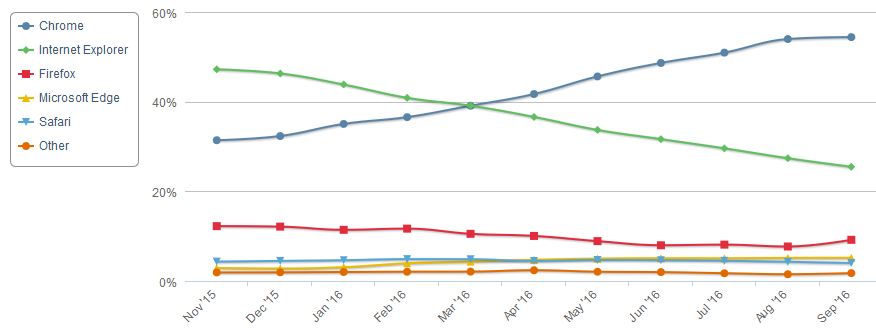
\includegraphics[width=1.1\textwidth]{marketshare.png}
	\caption{Marktaandeel van browsers op desktops\cite{NetShare}}
	\label{fig:marktaandeel}
\end{figure}
\newpage
\subsubsection{Speed of performance}
Google Chrome is snel in het gebruik, dit door de uitgebreide features die het de gebruiker makkelijker maken om eenvoudige acties uit te voeren. Denk bijvoorbeeld aan de lijst van veelbezochte sites bij het openen van een nieuwe tab (figuur \ref{fig:miniatuur}), het enorme aantal shortcuts\cite{shortcuts} en het automatisch aanvullen van URLs (figuur \ref{fig:autocomplete}). Bram merkt wel terecht op dat de flexibiliteit van Chrome door het toelaten van extensies hier wel een kostplaatje heeft: veel extensies vertragen Chrome aanzienelijk\cite{slow} en kunnen in sommige gevallen ook meer acties van de gebruiker verlangen.
\subsubsection{Rate of errors by users}
Een webbrowser wordt gebruikt om websites mee te navigeren, niet om je constant bezig te houden met errors. Hierom is het belangrijk dat Chrome er voor zorgt dat er zo weinig mogelijke errors mogelijk zijn. Hier slaagt Chrome goed in: wanneer bijvoorbeeld iets anders dan een URL ingegeven wordt in de adresbalk zal Chrome zoeken naar deze term (figuur \ref{fig:search}). Zelfs wanneer de gebruiker een fout maakt, is dit vaak makkelijk recht te zetten door gebruik te maken van knoppen als de vorige pagina knop, alsook toetsencombinatie zoals het sluiten van een tabblad ongedaan te maken. Ook hier is er weer de bedenking dat door het ondersteunen van extensies er vaker en meer uitgebreide fouten kunnen voorkomen, terwijl het basisproduct dit goed onder controle houdt.
\subsection{Ontwerpprincipes van Shneiderman}
\subsubsection{Herken de diversiteit}
Doordat Chrome gebruikt wordt door zo veel duizenden mensen, hebben we verschillende types gebruikers. We onderscheiden de beginners, de intermediate users en de expert users. Wij zijn het er over eens dat Chrome op iedere deelgroep goed inspeelt en zo niet alleen gebruikers wint, maar ze ook behoudt. Bij beginners komt dit door het feit dat deze browser zeer gelijkaardig is aan alle anderen, zo moeten ze niet veel leren als ze al een andere browser gebruiken. Er zijn weinig buttons, de UI is zeer simpel (figuur \ref{fig:smallUI}) en geeft duidelijke feedback aan de gebruiker wat altijd helpt (figuur \ref{fig:nocon}). Voor de intermediate gebruikers zijn er extensies om de browser naar wens te gebruiken, alsook het helpcentrum (figuur \ref{fig:helpcentrum}) waarin specifieke dingen makkelijk opgezocht kunnen worden.
\subsubsection{De acht gouden regels voor interface design}
\begin{itemize}
	\item Streven naar consistentie
	\newline
	De icoontjes van button zijn zeer consistent met andere browsers, zoals bijvoorbeeld Firefox (figuur \ref{fig:back}), ook werken de tabs en de adresbalk zoals andere browsers. In Chrome zelf worden telkens dezelfde grijstinten gebruikt, waardoor het een zeer samenhangende UI blijft.
	\item Frequente gebruikers toelaten schortcuts te gebruiken
	\newline
	Chrome biedt standaard een 50tal shortcuts aan\cite{shortcuts} en deze zijn uit te breiden door extensies. Dit is dan ook een klein minpuntje: om deze shortcuts uit te breiden zijn er extenties nodig want deze functionaliteit is niet inbegrepen in de standaard Chrome versie.
	\item Informatieve feedback aanbieden
	\newline
	Chrome geeft de gebruiker altijd informatieve feedback, dit kan men zien wanneer een pagina laadt: het standaard circeltje verschijnt. Ook bij het downloaden is er een duidelijke voortgangsbalk en bij het browsen in incognito komt niet alleen een melding in het groot tevoorschijn, maar ook de hele UI verandert van thema (figuur \ref{fig:incognito}).
	\item Dialogen ontwerpen zodat onverwachte resultaten uitgesloten worden en de voortgang duidelijk is
	\newline
	Chrome maakt af en toe gebruik van dit soort dialogen, maar dit blijkt wel een punt waar verbetering mogelijk is. Firefox bijvoorbeeld maakt hier vaker gebruik van, zo is er bij Chrome geen dialoog dat om bevestiging vraagt wanneer men het venster wil sluiten met meerdere tabbladen open, firefox doet dit wel. De dialogen die wel aanwezig zijn in Chrome, zijn wel zeer duidelijk en goed gemaakt, bekijk bijvoorbeeld de melding die gebruikers krijgen als ze een onveilige site willen bezoeken (figuur \ref{fig:privatecon}) of wanneer de gebruiker Chrome probeert te sluiten met een download actief (figuur \ref{fig:download}).
	\item Foutenpreventie
	\newline
	Er zijn weinig mogelijke fouten in een webbrowser, en zeker bij Chrome. Chrome zorgt ervoor dat de gebruiker weinig tijd verspilt aan het oplossen van fouten en laat de gebruiker toe gewoon door te surfen. Dit doet Chrome bijvoorbeeld door een zoekopdracht uit te voeren op inputs in de adresbar dat geen URLs zijn (figuur \ref{fig:search}).
	\item Acties omkeerbaar maken
	\newline
	In Chrome kunnen alle acties ongedaan gemaakt worden: denk maar aan het terug- of verdergaan in de browsergeschiedenis, alsook het ongedaan maken van het sluiten van tabbladen. Wat hier wel een minpunt is, is dat enkele van deze functies vast zitten achter shortcuts, die dus niet noodzakelijk bekend zijn en gebruikt worden door de gebruikers die nog geen expert zijn met Chrome, hierdoor gaat er dus een deel nuttige functionaliteit weg voor hen.
	\item Gebruiker meester over het systeem laten zijn
	\newline
	Door het bestaan van extensies (en de enorme hoeveelheid ervan\cite{extensions}) kan de gebruiker die dit wil zijn browser volledig aanpassen naar zijn of haar wensen. Denk bijvoorbeeld aan een Adblocker of zelfs userscripts: de gebruiker maakt van zijn browser wat hij wilt. Ook zijn er in Chrome zelf een groot aantal seettings die aangepast kunnen worden, maar daar staat tegenover dat enkele dingen (zoals bijvoorbeeld shortcuts) niet aangepast kunnen worden door de gebruiker.
	\item Gegevens beperken dat de gebruiker moet onthouden
	\newline
	De UI van Chrome is simpel en zeer gelijkaardig aan dat van andere browsers, waardoor het aantal zaken dat een gebruiker moet onthouden beperkt blijft. De enige zaken die echt onthouden moeten worden, zijn de shortcuts. Deze zijn echter vooral bedoeld voor de expertgebruikers, dus dit is geen probleem: van hen mag dit verwacht worden.
\end{itemize}
\newpage
\bibliographystyle{unsrt}
\bibliography{Taak_2}
\newpage

\end{document}

